\section{Identifying weakly-coupled carbon-pins}
This section will discuss the effect of dynamical decoupling on the interaction between the NV-center and weakly coupled nuclear spins.
This is used to explain the features in the fingerprint of \cref{fig:FP} and identify several nuclear spins.

\subsection{The effect of dynamical decoupling on nuclear spins}

During dynamical decoupling the electronic state alternates between the $m_s = 0$ and $m_s =+1$ state, this causes the nuclear spin to alternately rotate around two distinct quantization axes (\cref{fig:quantax}).
When the electron is in the $m_s=0$ state each nuclear spin precesses about $\bm{\omega_L}$ with the Larmor frequency given by \cref{eq:nuclear_larmor} .
When the electron is in the $m_s=+1$ state there is a hyperfine interaction between the nucleus and the NV-center (\cref{eq:nuclear_hamiltonian_1}) and the spin precesses around $\bm{\tilde{\omega}}=\bm{\omega_L} +\bm{A}$, where $\bm{A} = A_\parallel \bm{\hat{z}} + A_\perp \bm{\hat{x}}$ \citep{Taminiau2012Detection}.


\begin{figure}[htbp]
\centering

        \begin{tikzpicture}
            \node[anchor=south west,inner sep=0] at (0,0) {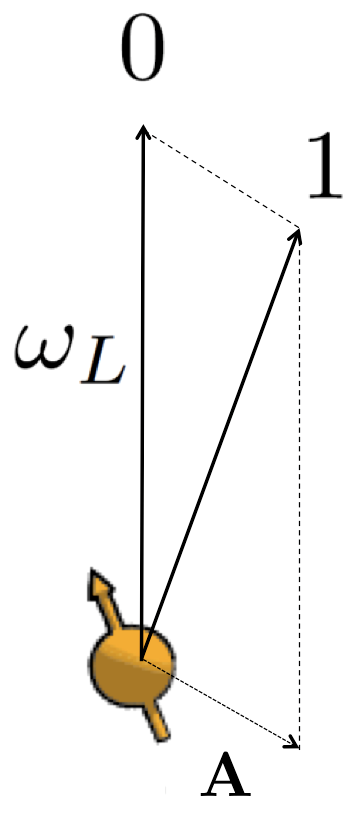
\includegraphics[keepaspectratio,width=0.15\textwidth]{./img/QuantizationAxis.png}};
            \node[font=\huge, text = black] at (1.6,2.0)  {${\tilde{\omega}}$};
        \end{tikzpicture}
\caption{Flipping the electron spin from the  $m_s=0$ to the $m_s= +1$ state changes the quantization axis of nuclear spins. For  $m_s=0$ all nuclear spins precess about $\bm{\omega_L}$. For  $m_s=+1$ each spin precesses about a distinct axis $\bm{\tilde{\omega}}=\bm{\omega_L} +\bm{A}$ due to the hyperfine interaction.}
\label{fig:quantax}
\end{figure}

The result of a decoupling sequence is a net rotation around an axis $\bm{\hat{\mathrm{n}}_i}$ by an angle $\theta$.
Where $\bm{\hat{\mathrm{n}}_i}$ depends on the initial state of the electron and $\theta$ is proportional to the number of pulses $N$ \citep{Taminiau2012Detection}.
$\bm{\hat{\mathrm{n}}_i} =\bm{\hat{\mathrm{n}}_0}$ when the electron starts in $m_s = 0$ and $\bm{\hat{\mathrm{n_i}}} =\bm{\hat{\mathrm{n}}_1}$ when the electron starts in $m_s = +1$.

\begin{figure}[htbp]
    \begin{subfigure}[t]{0.49\textwidth}\centering
        \centering
        \caption{}
        \includegraphics{Img/unCond_rot_taminiau.pdf}
        \label{fig:uncond_rot}
    \end{subfigure}
    \begin{subfigure}[t]{0.49\textwidth}\centering
        \centering
        \caption{}
        \includegraphics{Img/Cond_rot_taminiau.pdf}
        \label{fig:cond_rot}
    \end{subfigure}
    \caption{\subref{fig:uncond_rot} When the net rotation axes $\bm{\hat{\mathrm{n}}_0}$ and $\bm{\hat{\mathrm{n}}_1}$ point in the same direction the carbon experiences an unconditional rotation. \subref{fig:cond_rot} When the net rotation axes $\bm{\hat{\mathrm{n}}_0}$ and $\bm{\hat{\mathrm{n}}_1}$ are anti-parallel the carbon experiences a conditional rotation, either around $+x$ or $-x$. Figure from \citet{Taminiau2012Detection}.}
    \label{fig:conditional_and_unconditional_rotation}
\end{figure}

When the net rotation axes point in a different direction a conditional operation is executed during dynamical decoupling (\cref{fig:conditional_and_unconditional_rotation}).
In a dynamical decoupling spectroscopy contrast is lowered when a conditional operation is executed.
To understand when this occurs it is useful to consider three different cases.
A weakly coupled carbon spin in: the trivial regime where $A_\perp=0$, the basic regime where $A_\perp \ll \omega_L$ and the complex regime where $A_\perp \sim \omega_L$.
For a mathematical description of the result of a dynamical decoupling spectroscopy the reader is referred to \cref{sec:mathematical_description_dd_spectro}.

\subsubsection{The trivial regime ($A_\perp=0$)}
Because there is no orthogonal component of the hyperfine the spin will precess around the $z$-axis independent of the initial electronic spin-state.
Therefore the operation not conditional and no signal for such spins is observed in a dynamical decoupling spectroscopy.

\subsubsection{The basic regime ($A_\perp \ll \omega_L$)}
In the basic regime the net rotation axes are practically parallel and point in the $z$-direction for almost every $\tau$ except for a specific resonant condition for which the axes are anti-parallel.
This resonant condition is given by \cref{eq:res_dip_loc}:
 \begin{equation}
\tau = \frac{(2k+1)\pi}{2 \omega_L + A_\parallel}
\label{eq:res_dip_loc}
\end{equation}
Where $k$ is an integer, and has a Lorentzian shape in a dynamical decoupling spectroscopy.
These sharp resonances are the origin of the sharp dips in the dynamical decoupling spectroscopy.
The FWHM of the resonance is given by \cref{eq:res_dip_width}:
 \begin{equation}
\mathrm{FWHM_{DD}} = \frac{A_\perp}{2 \omega_L^2}
\label{eq:res_dip_width}
\end{equation}


\subsubsection{The complex regime ($A_\perp \sim \omega_L$)}

In the case where $\bm{\omega_L}$ and $\bm{A_\perp}$ are of comparable magnitude the net rotation axes are strongly dependent on the initial electron-state for almost any $\tau$.
When a carbon is in this regime it is no longer possible to describe it as a narrow resonance in the dynamical decoupling spectroscopy.
The response is visible as a wide resonance with an oscillation on top of it, spin 3 in \cref{fig:FP} is an example of such a spin.

\paragraph{ }
When the response of multiple carbon spins in a dynamical decoupling spectroscopy overlaps, the electron performs an entangling operation on all these carbons.
Because of this the measured contrast in a dynamical decoupling spectroscopy goes down rapidly when the responses of multiple carbons overlap.
This makes it hard to resolve individual spins when a spin has a broad response, such as a spin in the complex regime, or if there are several spins with similar hyperfine couplings.


\subsection{Identifying Individual Carbon-spins}
Using the previous section we will look at \cref{fig:FP} in greater detail.

A broad collapse of the signal is clearly visible around $\tau/(4\tau_L) = m$ for odd $m$.
This broad collapse is caused by the response of multiple spins overlapping.

At the edges of this collapse several sharp dips are visible.
These correspond to individual spins.
A first estimate of the hyperfine coupling to these spins can be made based on their location and width using \cref{eq:res_dip_loc,eq:res_dip_width}.

Between the broad collapses there alternately appears an oscillation.
This oscillation is caused by a spin in the complex regime.
Its position can be used to get a rough estimate for its hyperfine coupling.

By computing the responses for the hyperfine parameters using \cref{eq:contrast_single_carbon_spin} a more accurate estimation was made.
13 distinct carbon spins were identified.

The parameters of the 4 strongest coupled carbons are listed in \cref{tbl:HF_par} and their computed responses are visible as colored lines in \cref{fig:FP}.
All estimated hyperfine parameters and a link to the full dynamical decoupling dataset can be found in \cref{chap:Fingerprint_data_appendix}.

\begin{table}[htbp]
\centering
    \caption{Estimated hyperfine parameters for spins 1 to 4 in \cref{fig:FP}.}
    \begin{tabular}{cllll}
    Carbon & \quad \quad  $A_{\parallel} $ & \quad \quad $A_{\perp}$ \\ \hline
    1         & $2 \pi \cdot${ }30.0 kHz             & $2 \pi \cdot${ }80.0 kHz                \\
    2         & $2 \pi \cdot${ }27.0 kHz             & $2 \pi \cdot${ }28.5 kHz              \\
    3         & $2 \pi \cdot$-51.0 kHz          & $2 \pi \cdot$105.0 kHz              \\
    4         & $2 \pi \cdot${ }45.1 kHz           & $2 \pi \cdot${ }20.0 kHz                \\
    \end{tabular}
    \label{tbl:HF_par}
\end{table}

